\section{Anforderungen}
Das Rahmenwerk dient der Vereinfachung des Entwicklungsprozesses.
Je nach Anwendung sind von diesem verschiedene Anforderungen zu erfüllen, daher ist die Wahl des richtigen Rahmenwerks besonders wichtig.
Dieser Abschnitt beschäftigt sich mit dem Vergleich der einzelnen Möglichkeiten, sowie einer endgültigen Auswahl eines der Rahmenwerke zur Verwendung im Diplomprojekt.
Die geforderten Funktionen für dieses Projekt beinhalten:
\begin{itemize}
    \item eine einfache Möglichkeit der Multiplattform-Entwicklung der App. Wenn möglich soll nur eine App geschrieben werden, die dann auf allen Zielplattformen (Android, iOS) lauffähig ist.
    \item Die Programmierung sollte in einer bereits bekannten Programmiersprache möglich sein.
    Für die Fachrichtung Elektrotechnik der HTL Anichstraße werden momentan die Sprachen C, C++ und C\#, in untergeordnetem Ausmaß auch JavaScript für Webseiten-Entwicklung unterrichtet.
    \item Das Rahmenwerk und die dazugehörige Entwicklungsumgebung sollten für nichtkommerzielle Anwendungen wie diese Diplomarbeit frei zur Verfügung stehen.
    \item Die Entwicklungswerkzeuge sollten das Windows-, optional das Linux-Betriebs\-sys\-tem unterstützen.
\end{itemize}

\section{Vergleich}
Für die App-Programmierung stehen viele verschiedene Rahmenwerke bereits zur Verfügung.
\subsection{Microsoft Xamarin}
ist ein Rahmenwerk, mit dem man Multiplattform-Applikationen für unter Anderem Android, iOS, \ac{uwp} und noch viele weitere Plattformen erstellen kann.
Es basiert auf Microsofts \ac{dotnet} und dem Mono-Projekt, welches sich als Ziel gesetzt hat, das \ac{dotnet} auf andere Plattformen zu portieren.
Xamarin bietet mehrere Projekttypen an, darunter Xamarin.Android und Xamarin.iOS für native App-Entwicklung und Xamarin.Forms für großteils plattformunabhängige Entwicklung.
Eine Xamarin.Forms-Solution besteht daher aus mehreren Teilen:
\begin{itemize}
    \item Portable/\acs{dotnet}-Standard Projekt, das den plattformunabhängigen Code beinhält
    \item natives Xamarin-Projekt für jede Zielplattform
\end{itemize}
Der Vorteil Xamarins ist, dass der Großteil des geschriebenen Codes im plattformunabhängigen Projekt bleibt und nur für wenige Funktionen auf native Programmierung zurückgegriffen wird, wie zum Beispiel für hardwarenahe Audio-Aufnahme.
Außerdem ist das Xamarin-Projekt Open-Source, das bedeutet jeder kann den Quellcode betrachten und unter Umständen Verbesserungen vorbringen.
Zusätzlich ist es für diese Anwendung kostenfrei.

\subsection{Webtechnologiebasierte Rahmenwerke}
In dieser Kategorie existieren sehr viele verschiedene Rahmenwerke, darunter Apache Cordova, Adobe PhoneGap, sowie Facebook React Native.
Am Beispiel von Apache Cordova werden hier die Vor- und Nachteile dieses Ansatzes erläutert.

%quelle
Cordova ist ein App-Entwicklungs-Rahmenwerk welches ursprünglich von der Firma Nitobi unter dem Name PhoneGap entwickelt wurde.
Im Jahr 2011 wurde Nitobi von Adobe aufgekauft.
Später wurde neben der Closed-Source-Version auch eine quelloffene Version unter dem Namen Cordova veröffentlicht. \cite{adobe-phonegap}\par

Apps werden mittels gängiger Webtechnologie, wie zum Beispiel JavaScript, \acs{css} und Ähnlichen, entwickelt und realisiert, weshalb das Rahmenwerk alle gängigen Plattformen unterstützt.
Der Vorteil von Cordova und ähnlichen Rahmenwerken liegt im enormen Support dieser Webtechnologien, jedoch sind Sprachen wie JavaScript für Back-End-Programmierung weniger geeignet.
Noch dazu kommt, dass an der HTL Anichstraße großteils die Programmierung nur in C und C\# gelehrt wird, weshalb die Entwicklung mit JavaScript im vereinbarten Zeitrahmen der Diplomarbeit nicht realistisch umsetzbar ist.

Aufgrund der oben erläuterten Vor- und Nachteile der möglichen Ansätze wurde die Verwendung von Xamarin für diese Diplomarbeit festgelegt.

\section{Build-Umgebung}
\subsection{Visual Studio 2019}
Aufgrund obiger Aufstellung wurde Visual Studio 2019 der Firma Microsoft als Entwicklungsumgebung gewählt.
Visual Studio ist das offizielle Werkzeug für die Programmierung mit dem Xamarin-Rahmenwerk und die wahrscheinlich bestbekannte Entwicklungsumgebung überhaupt.
Die Community-Edition für Schüler und Private steht gratis zum Download zur Verfügung.
Diese beinhält alle wichtigen Entwicklungswerkzeuge wie zum Beispiel die automatische Code-Vervollständigung.
Für die Nutzung wird nach den ersten 30 Tagen ein Microsoft-Konto benötigt.\par
%versionsvergleich hier https://visualstudio.microsoft.com/vs/compare/

Der Programmcode wird von Visual Studio 2019 in sogenannten Solutions organisiert.
Am Beispiel einer Xamarin.Forms-Applikation lässt sich das sehr gut erläutern;
die Solution enthält auf oberster Ebene drei Projekte: das portable Projekt, das Android- und das iOS-Projekt.
Ein Projekt kann bereits für sich lauffähig oder nur Teil eines größeren Programms sein.\par

Visual Studio 2019 unterstützt viele verschiedene Einsatzbereiche, die bei der Installation ausgewählt werden müssen.
Eine volle Installation mit allen Funktionen und Projektarten ist zwar möglich, benötigt allerdings bis zu 210GB Speicherplatz des Systems.
Eine typische Xamarin-Installation benötigt etwa 6.25GB Festplattenspeicher.
Für eine solche Installation muss im Visual Studio Installer das \enquote{Mobile development with \acs{dotnet}}-Paket ausgewählt und installiert werden.
\begin{figure}[H]
    \centering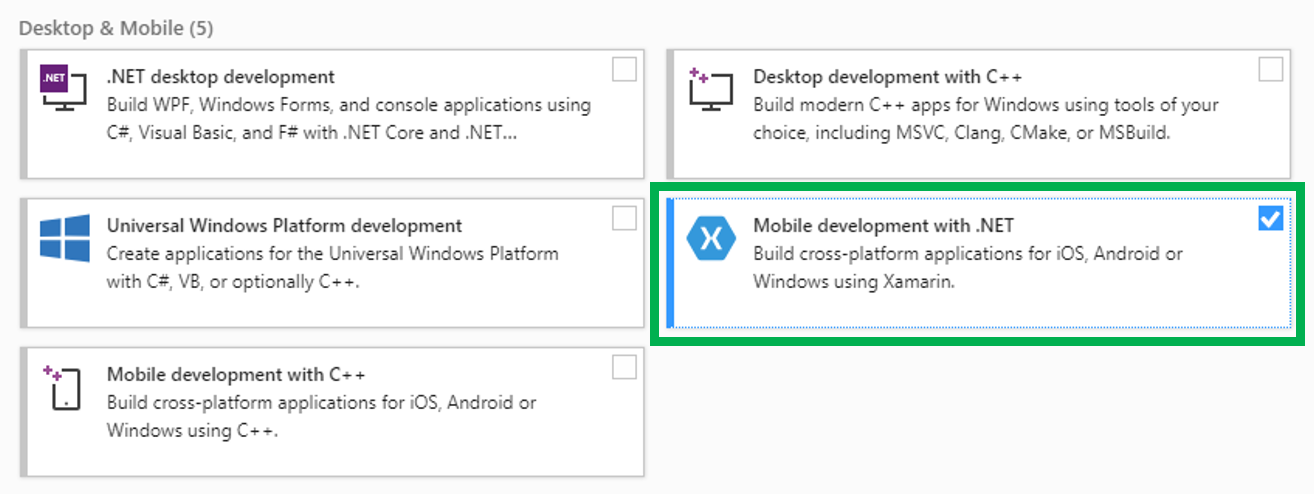
\includegraphics[width=0.9\linewidth]{images/auswahl_rahmenwerk/installation.png}    
    \caption{Auswahl des Xamarin-Rahmenwerks bei der Installation}
\end{figure}
Es empfiehlt sich, das Paket für \enquote{\acs{dotnet} desktop development} dazu zu installieren, damit neue, noch nicht bekannte \ac{dotnet}-Technologien in einer einfacheren Konsolen-Anwen\-dung ausprobiert werden können.
Das Paket benötigt ungefähr weitere 0.8GB.\par
Auf nähere Details der Installation von Visual Studio wird hier nicht eingegangen, diese können aber auf der Microsoft-Dokumentationsseite \cite[vgl.][]{msdoc-vs-install} nachgeschlagen werden.
%Betriebssystem, Hardwareanforderungen
%
\subsection{Android \acs{sdk}}
Um Xamarin-Applikationen für Android-Geräte entwickeln zu können wird das von Google bereitgestellte Android \ac{sdk} benötigt, um das Programm in ein \ac{apk} umzuwandeln. Die einzelnen Komponenten können im Android-\ac{sdk}-Manager des Visual Studio installiert werden.
Dieser ist im Menüband unter \enquote{Tools\textbackslash Android\textbackslash Android \ac{sdk} Manager} zu finden.
\begin{figure}[H]
    \centering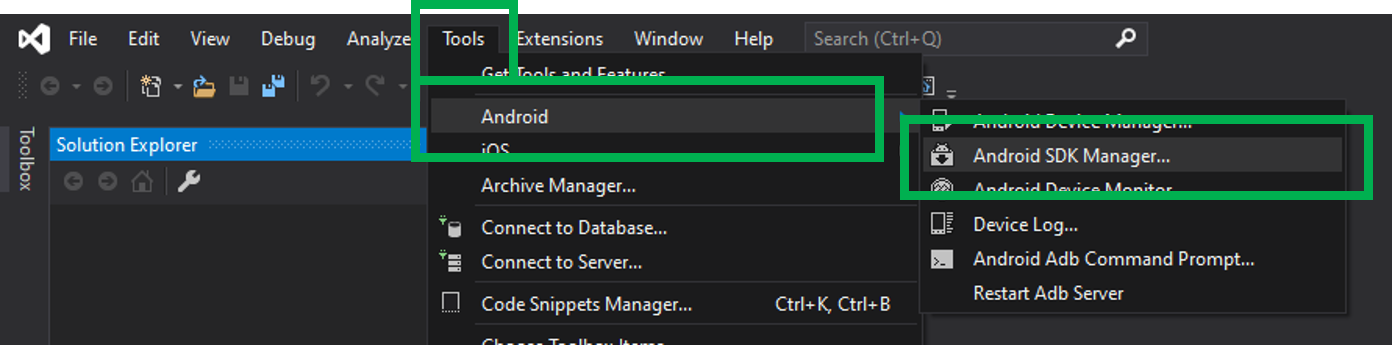
\includegraphics[width=0.9\linewidth]{images/auswahl_rahmenwerk/android_sdk_installation.png}    
    \caption{Android \acs{sdk} Manager}
\end{figure}
Der \ac{sdk}-Manager ist in zwei Seiten unterteilt - \enquote{Platforms} und \enquote{Tools}.\par

Auf der \enquote{Plat\-forms}-Seite können die benötigten \ac{sdk}-Teile für jede Android-Version installiert werden.
Benötigt wird nur die Version, mit der das Projekt später kompiliert werden soll.
Außerdem kann man auf dieser Seite des \ac{sdk}-Managers System-Abbilder für den Android Emulator installieren.\par

Über die \enquote{Tools}-Seite können verschiedenste Entwicklungswerkzeuge installiert werden.
Grundsätzlich erforderlich sind \enquote{Android \acs{sdk} Tools}, \enquote{Android \acs{sdk} Platform Tools} und \enquote{Android \acs{sdk} Build Tools} um Android-Apps mit Xamarin entwickeln zu können.
Für dieses Projekt werden Push-Benachrichtigungen via Google Cloud Messaging verwendet, daher werden noch zusätzlich die Pakete für die \enquote{Google Play Services} sowie die \enquote{Google Cloud Messaging for Android Library} installiert.
Wie Push-Benachrichtigungen genauer funktionieren wird später im Kapitel \crossref{ch:push} auf Seite \pageref{ch:push} behandelt.
\begin{figure}[H]
    \centering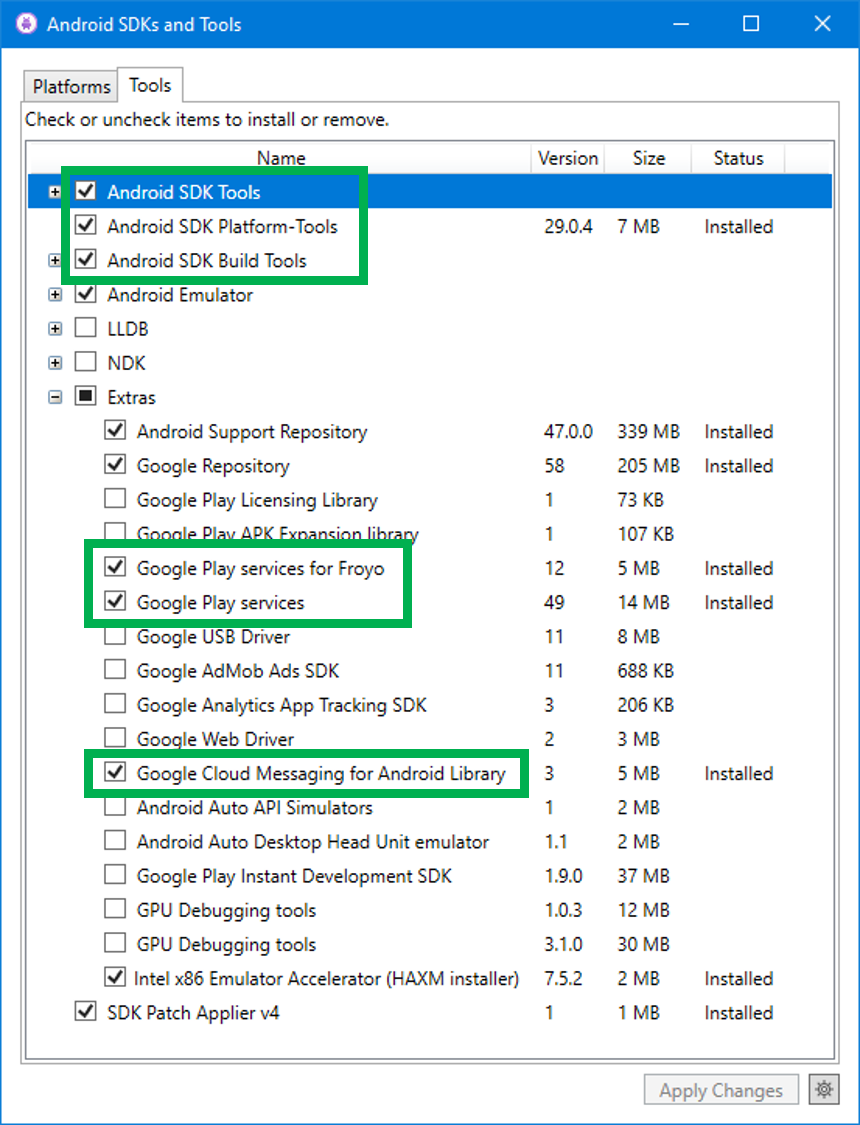
\includegraphics[width=0.8\linewidth]{images/auswahl_rahmenwerk/android_sdk_auswahl.png}    
    \caption{Notwendige Teile des Android \acs{sdk}}
\end{figure}

\subsection{Build-Vorgang}
Um den geschriebenen Code in eine lauffähige Applikation umzuwandeln wird ein sogenannter Compiler benötigt.
Die Aufgabe des Compilers ist es, die geschriebene Hochsprache entweder direkt in \acs{cpu}-Maschinensprache bzw. eine Art Zwischencode zu kompilieren, d.h. umzuwandeln. Im Fall einer einfachen C\#-Konsolenanwendung ist der Build-Vorgang noch relativ simpel:
\begin{enumerate}
    \item Alle einzelnen Code-Dateien werden nacheinander vom Compiler in \ac{cil}, eine Zwischensprache des \ac{dotnet}, umgewandelt.
    \item Der Linker fügt die einzelnen Teile zu einem Gesamten zusammen.
    Das Resultat ist eine Datei, die wie eine ausführbare .EXE-Datei erscheint.
    \item Wenn das zusammengefügte Programm gestartet wird, kompiliert die \ac{clr} den Zwischencode in ausführbaren Maschinen-Code.
    Die \acs{cpu} des Systems kann diesen dann ausführen.
\end{enumerate}
\begin{figure}[H]
    \centering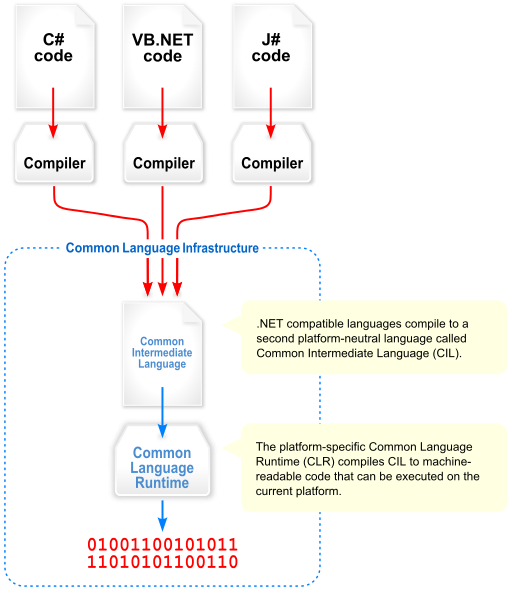
\includegraphics[height=12cm]{images/auswahl_rahmenwerk/dotnet-compilation.png}
    \caption{Build-Vorgang einer \ac{dotnet}-Applikation\cite{wiki-cli}}
    %\footfullcite[]{wiki-cli}
\end{figure}

Ähnlich funktioniert dieser Vorgang auch bei einer Xamarin.Forms-App, allerdings wesentlich komplexer.
Eine Xamarin.Forms-Solution besteht aus drei Einzel-Projekten (PiBell, PiBell.Android, PiBell.iOS), wobei das \acs{dotnet}-Standard-Projekt als Teil der anderen zwei verbaut werden muss.
Dadurch ergibt sich ein in Abbildung \crossref{fig:build-forms} dargestellter Build-Vorgang.
\begin{figure}
    \centering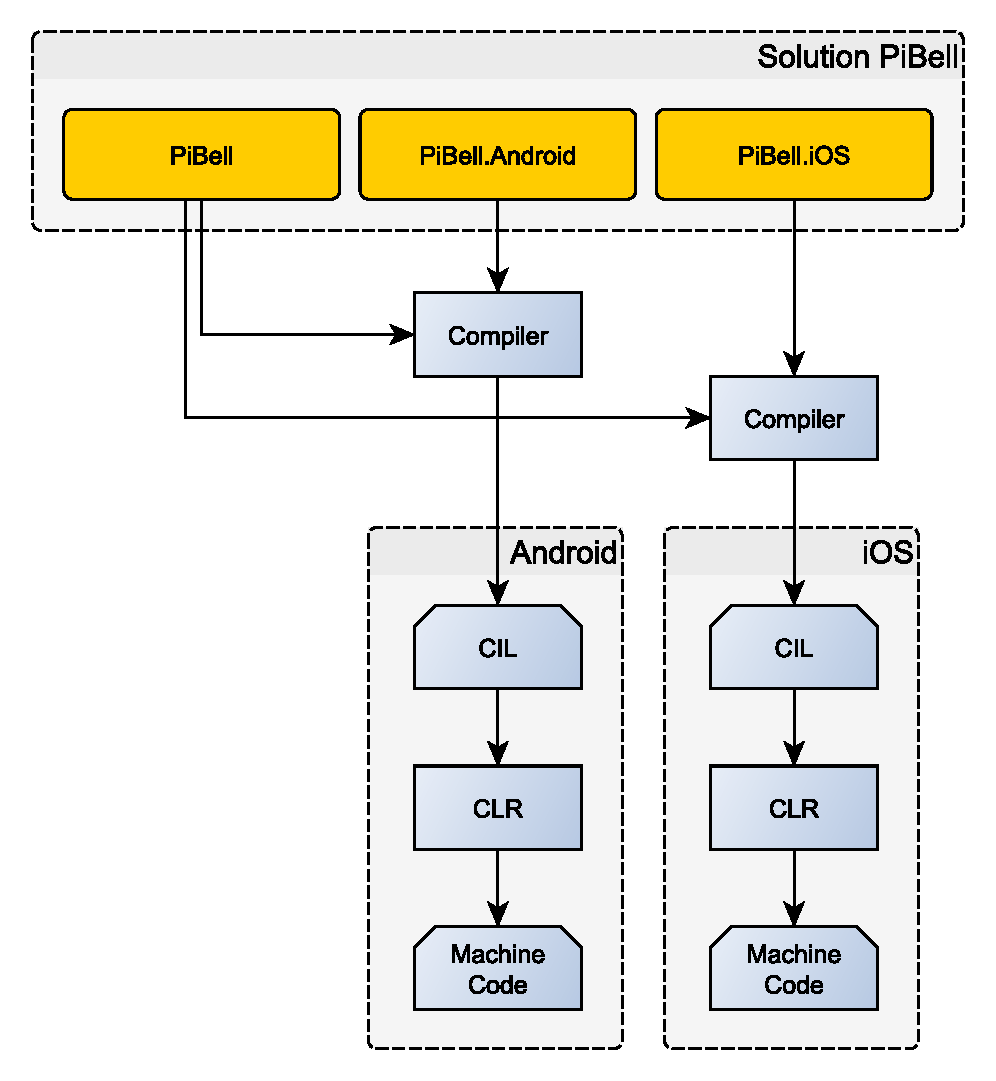
\includegraphics[width=0.9\linewidth]{images/auswahl_rahmenwerk/build-vorgang.pdf}
    \caption{Build-Vorgang einer Xamarin.Forms-Solution}
    \label{fig:build-forms}
\end{figure}

%Weg vom Programm zur binary
%microsoft VS2019
%frei zugänglich
%nur auf windows, kein linux-support
%...